\documentclass[logo,reportComp]{thesis}
\usepackage[cpp,linenum]{mypackage}

\title{计算机网络实验报告}
\subtitle{实验四:应用层实验}
\school{数据科学与计算机学院}
\author{陈鸿峥}
\classname{17大数据与人工智能}
\stunum{17341015}
\headercontext{计算机网络实验报告}

\begin{document}

\maketitle

\section{实验目的}
掌握应用层的基本工作原理和实现方法。

\section{实验工具}
Telnet或SecureCRT

\section{实验环境}
本机为Ubuntu 18.04 (LTS) + gcc 7.3.0

\section{注意事项}
\begin{itemize}
    \item 截屏时注意遮盖掉自己的邮箱密码
    \item QQ邮箱需要在Web访问方式下开启POP3和SMTP服务才允许在客户端访问(设置/账号/开启POP3/SMTP),否则会出现错误``454 Authentication failed, please open smtp flag first!''
    \item QQ邮箱的接收邮件服务器:pop.qq.com,端口号为995
    \item QQ邮箱的发送邮件服务器:smtp.qq.com,端口号为465
    \item 客户端登录的用户名为QQ号的base64编码
    \item 客户端登录的密码也采用base64编码
\end{itemize}

\section{实验内容}
先认真阅读课件\verb'Chapter2-applicaton-layer.pdf',再完成下面内容。
注意:协议标准可以查阅RFC;选取的内容不要与课件相同;响应内容太长时自己选取截取前后部分以及其中重点部分。

参考视频:\url{http://172.18.187.9/video/}

(选做)使用自己编写的TcpClient运行步骤一$\thicksim$步骤四,具体见步骤六。

如果不自己编写TcpClient,可以尝试使用老师给的\verb'TcpClient.exe'完成步骤一$\thicksim$步骤四,如果不愿意尝试,可以使用telnet来完成实验。

\subsection{HTTP协议}
看完HTTP协议的课件后完成以下实验。
\begin{enumerate}
    \item 从学院网站(\url{sdcs.sysu.edu.cn})找一网页下载。\\
http请求:
\begin{lstlisting}
GET /content/3822 HTTP/1.1
Connection:close
Host:sdcs.sysu.edu.cn
\end{lstlisting}
http响应:
\begin{figure}[H]
\centering
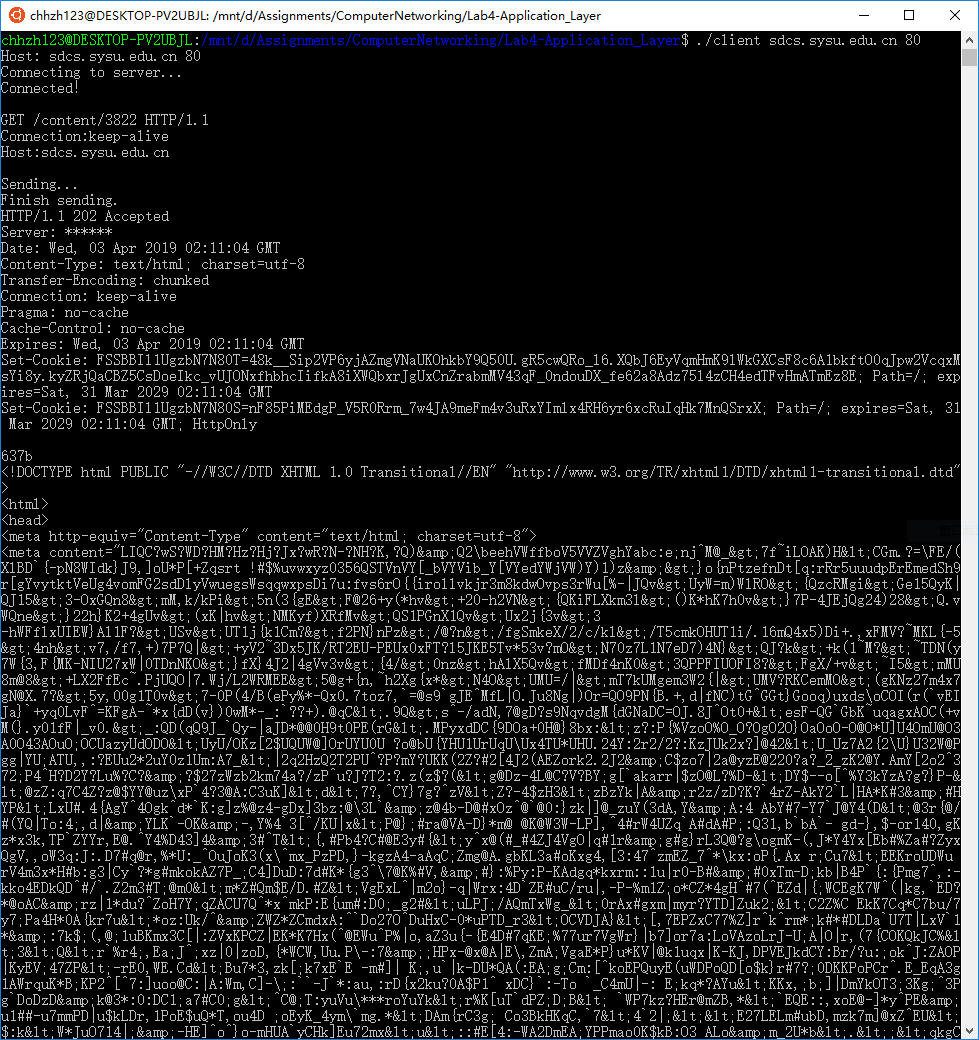
\includegraphics[width=0.8\linewidth]{fig/http-1.PNG}
\caption{下载学院网站}
\label{fig:http-1}
\end{figure}
    \item 从学院网站(\url{sdcs.sysu.edu.cn})找一图片下载。\\
http请求:
\begin{lstlisting}
GET /sites/sdcs.sysu.edu.cn/files/u191/12_2.jpg HTTP/1.1
Connection:close
Host:sdcs.sysu.edu.cn
\end{lstlisting}
http响应:
\begin{figure}[H]
\centering
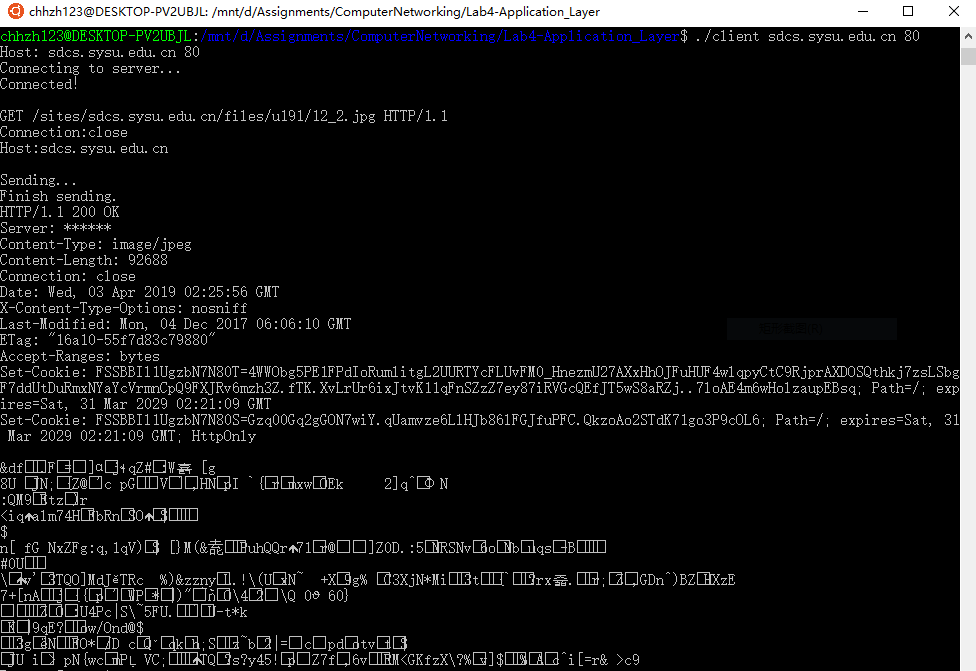
\includegraphics[width=0.8\linewidth]{fig/http-2.PNG}
\caption{下载学院图片}
\label{fig:http-2}
\end{figure}
    \item 在http请求的头部行中加入\verb'If-Modified-Since: Fri, 16 Jan  2019 13:22:17 GMT'从学院网站下载(2)的图片。\\
    \textbf{注意Linux的编码与Windows编码存在差异,使用Linux客户端可能无法正常显示图片编码!(这与Linux内置的telnet客户端相同)}\\
http请求:
\begin{lstlisting}
GET /sites/sdcs.sysu.edu.cn/files/u191/12_2.jpg HTTP/1.1
Connection:close
Host:sdcs.sysu.edu.cn
If-Modified-Since: Fri, 16 Jan  2019 13:22:17 GMT
\end{lstlisting}
http响应:
\begin{figure}[H]
\centering
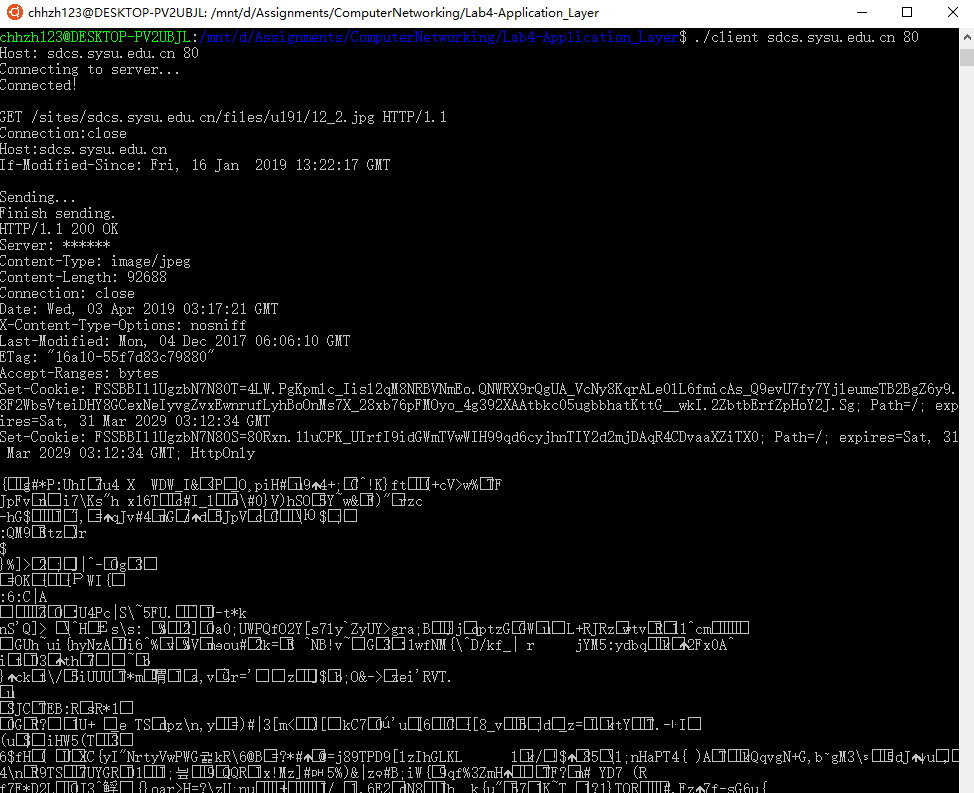
\includegraphics[width=0.8\linewidth]{fig/http-3.PNG}
\caption{下载学院图片2}
\label{fig:http-3}
\end{figure}
    \item 用流水线方式实现前面的(1)(2),即把它们的请求拷贝到一起后发送出去(可能太长,第一部分可以只看到末尾)。\\
http请求:
\begin{lstlisting}
GET /content/3822 HTTP/1.1
Connection:keep-alive
Host:sdcs.sysu.edu.cn

GET /sites/sdcs.sysu.edu.cn/files/u191/12_2.jpg HTTP/1.1
Connection:keep-alive
Host:sdcs.sysu.edu.cn
\end{lstlisting}
http响应:注意两条回复的消息以HTTP为分隔
\begin{figure}[H]
\centering
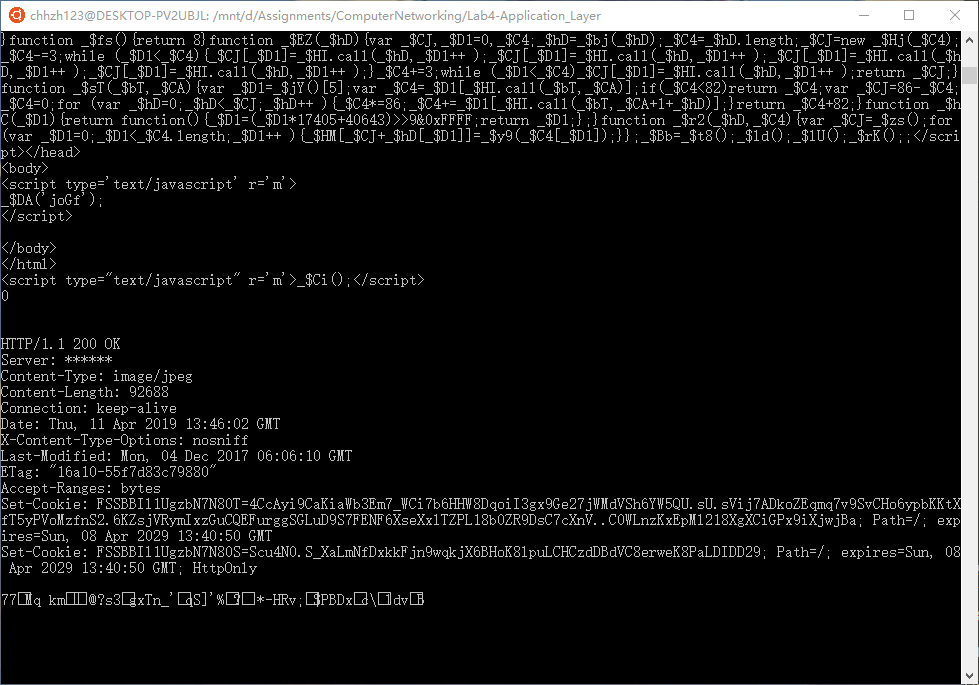
\includegraphics[width=0.8\linewidth]{fig/http-4.PNG}
\caption{流水线HTTP}
\label{fig:http-4}
\end{figure}

\end{enumerate}

\subsection{FTP协议}
看完FTP协议的课件后完成以下实验(测试服务器上的目录结构和文件见``参考资料'')。
\par FTP服务器:IP地址为172.18.187.10,端口号为 21 (用户名:abc,密码:123666)
\begin{enumerate}
\item 上传用学号命名的一个文本文件(学号\verb'.txt')\\
控制连接的请求响应信息:
\begin{figure}[H]
\centering
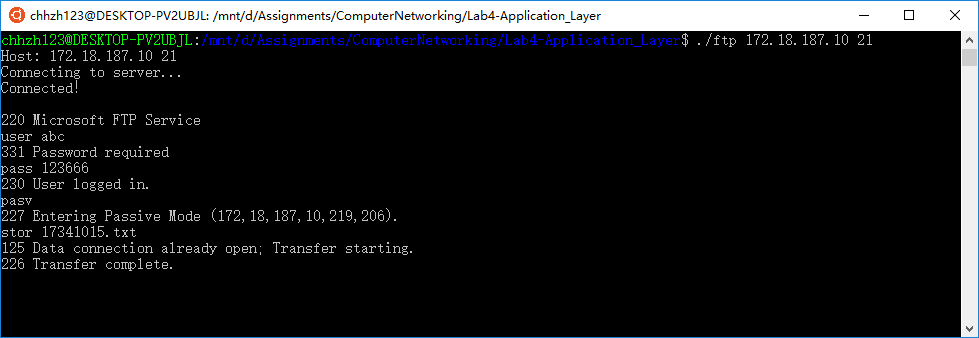
\includegraphics[width=0.8\linewidth]{fig/ftp-00.PNG}
\end{figure}

数据连接的截屏:
\begin{figure}[H]
\centering
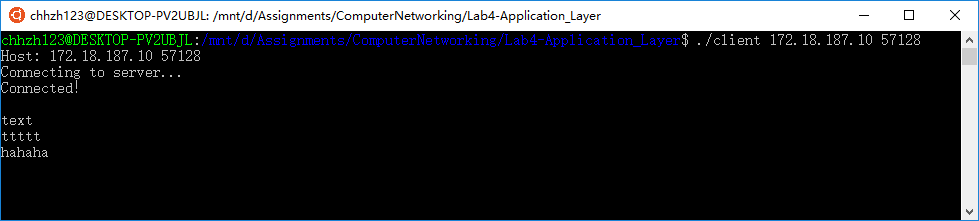
\includegraphics[width=0.8\linewidth]{fig/ftp-01.PNG}
\end{figure}

\item 查看当前目录内容(太多则选择一些),并标注出(1)中自己上传的文件\\
控制连接的请求响应信息:
\begin{figure}[H]
\centering
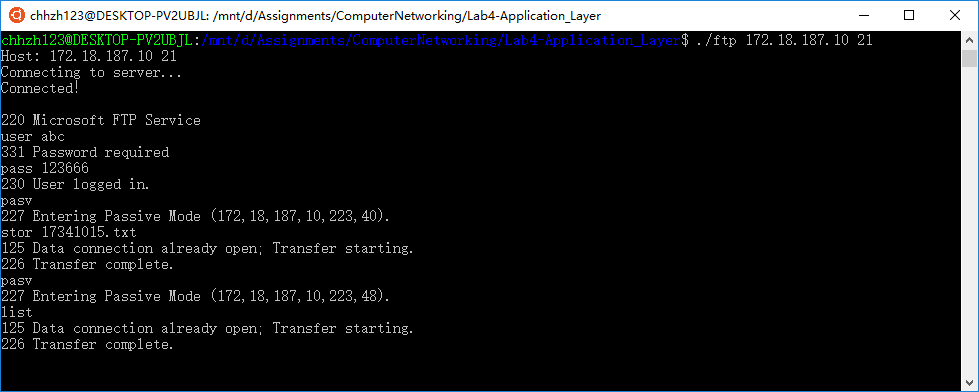
\includegraphics[width=0.8\linewidth]{fig/ftp-10.PNG}
\end{figure}

数据连接的截屏:
\begin{figure}[H]
\centering
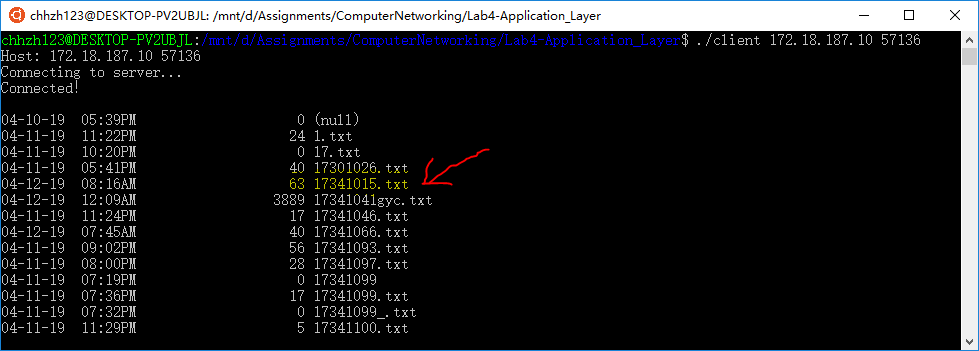
\includegraphics[width=0.8\linewidth]{fig/ftp-11.PNG}
\end{figure}

\item 下载(1)中自己上传的文本文件\\
控制连接的请求响应信息:
\begin{figure}[H]
\centering
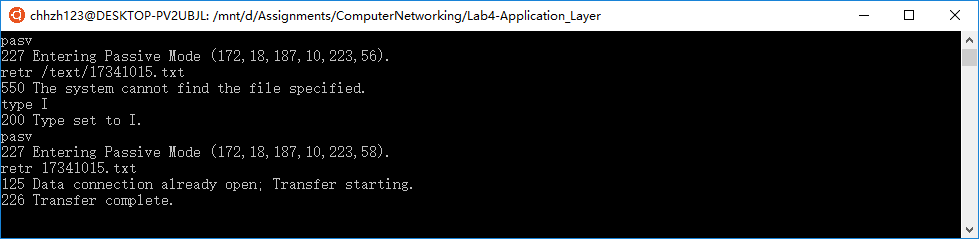
\includegraphics[width=0.8\linewidth]{fig/ftp-20.PNG}
\end{figure}

数据连接的截屏:
\begin{figure}[H]
\centering
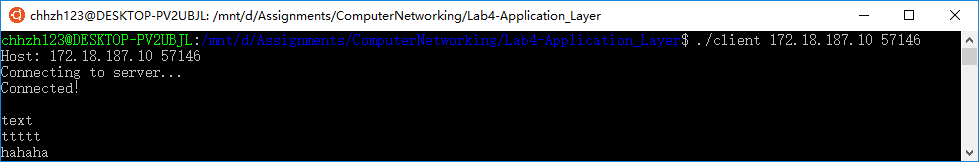
\includegraphics[width=0.8\linewidth]{fig/ftp-21.PNG}
\end{figure}

\item 下载\verb'/ebook'下的一个二进制文件(例如\verb'.pdf'文件)\\
控制连接的请求响应信息:
\begin{figure}[H]
\centering
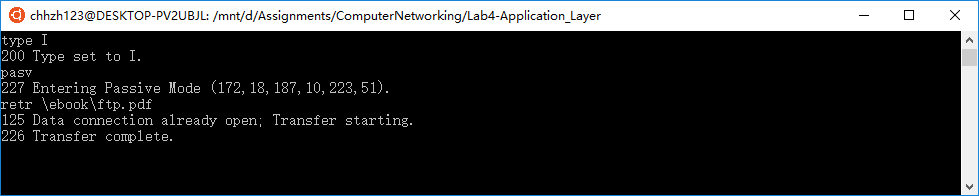
\includegraphics[width=0.8\linewidth]{fig/ftp-30.PNG}
\end{figure}

数据连接的截屏:
\begin{figure}[H]
\centering
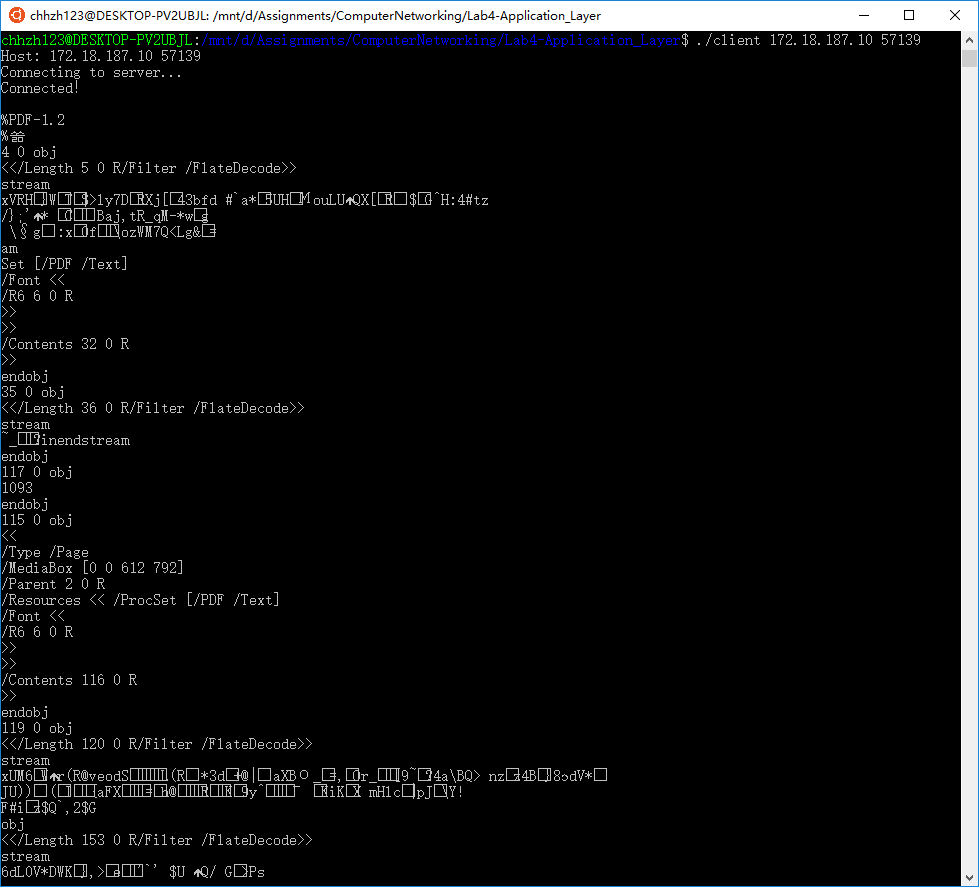
\includegraphics[width=0.8\linewidth]{fig/ftp-31.PNG}
\end{figure}

\item 采用断点续传下载一个\verb'/text'下的一个文本文件的一部分\\
控制连接的请求响应信息:
\begin{figure}[H]
\centering
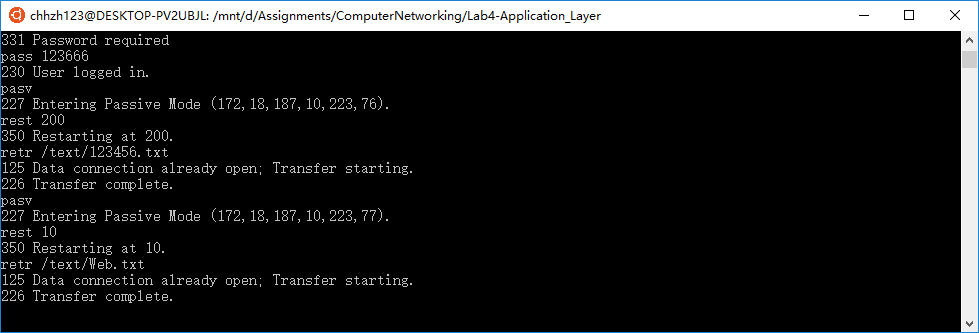
\includegraphics[width=0.8\linewidth]{fig/ftp-40.PNG}
\end{figure}

数据连接的截屏:
\begin{figure}[H]
\centering
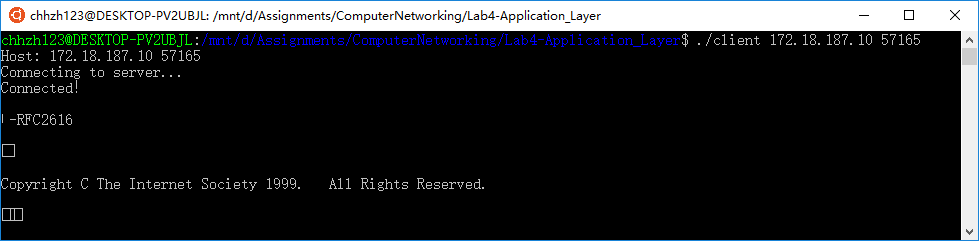
\includegraphics[width=0.8\linewidth]{fig/ftp-41.PNG}
\end{figure}

\end{enumerate}

\subsection{SMTP协议}
看完SMTP协议的课件后做以下实验。
\par 邮箱\verb'zsusender3@sina.com'的用户名\verb'zsusender3',密码:\verb'123456Aa'。
\par \textbf{由于老师的邮箱已被查封,因而采用自己的网易163邮箱,向QQ邮箱发信。}
\begin{enumerate}
\item 通过\verb'zsusender3@sina.com'发一封没有附件的邮件到你的邮箱。
注意更改时间为当前时间。\\
请求和响应信息:
\begin{figure}[H]
\centering
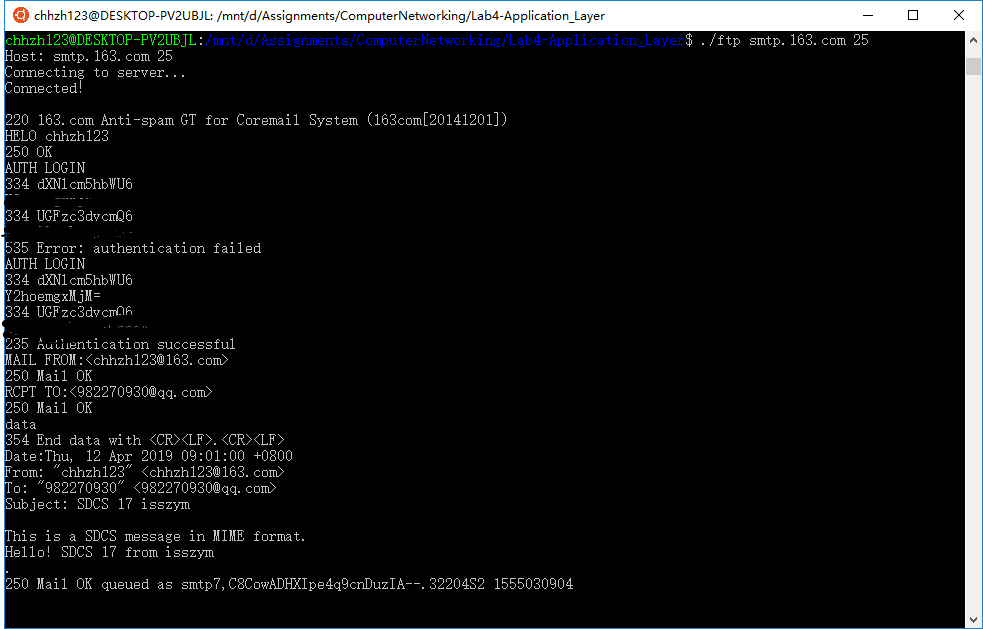
\includegraphics[width=0.8\linewidth]{fig/smtp-1.PNG}
\end{figure}
\begin{figure}[H]
\centering
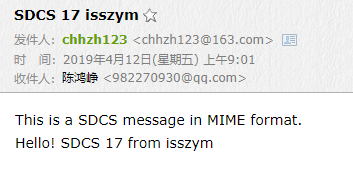
\includegraphics[width=0.2\linewidth]{fig/smtp-11.PNG}
\end{figure}

\item 通过\verb'zsusender3@sina.com'发一封带附件(二进制文件)的邮件(\verb'MIME.txt')到你的邮箱。
参考课件\verb'MIME.pdf'和观看MIME的视频。\\
请求和响应信息:
\begin{figure}[H]
\centering
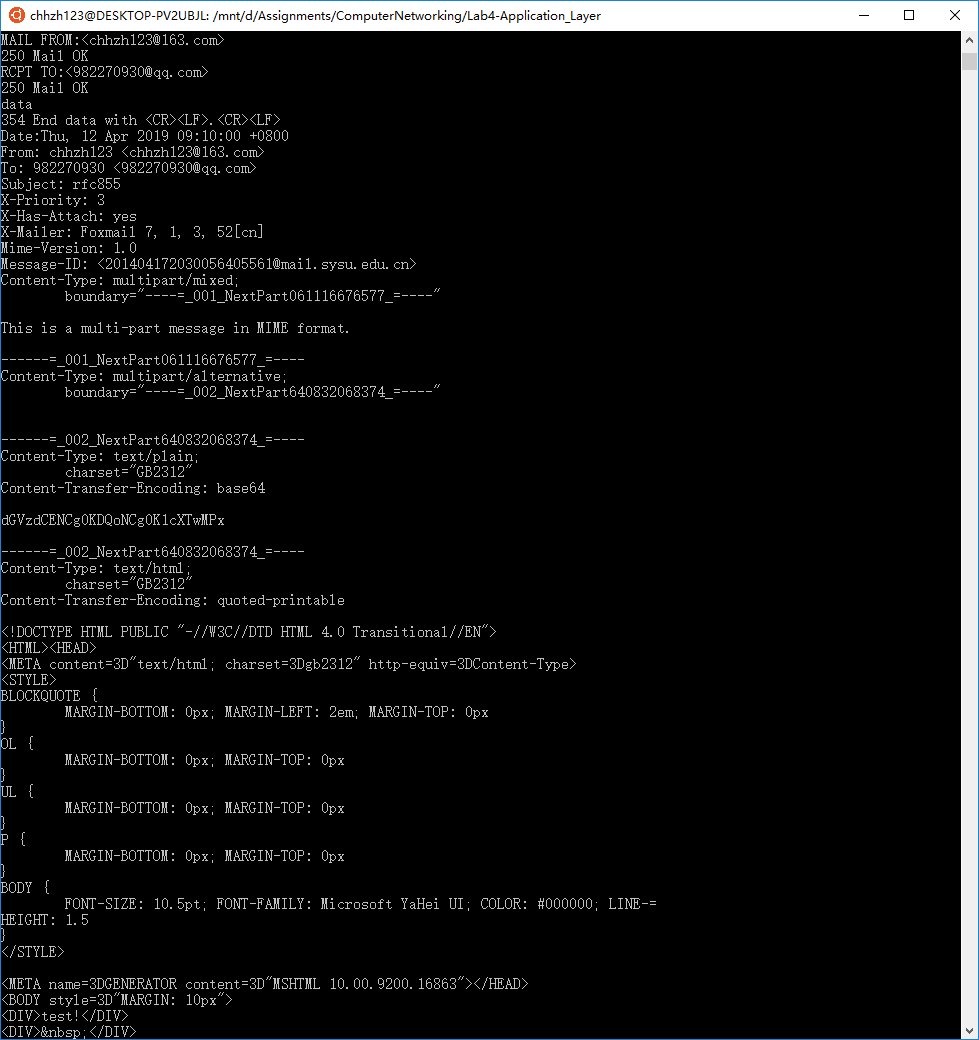
\includegraphics[width=0.8\linewidth]{fig/smtp-2.PNG}
\end{figure}
\begin{figure}[H]
\centering
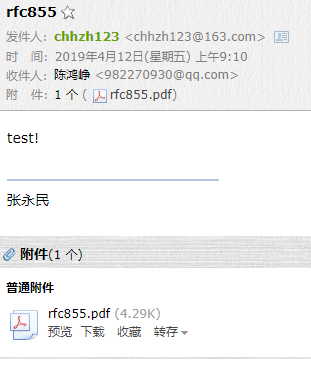
\includegraphics[width=0.2\linewidth]{fig/smtp-21.PNG}
\end{figure}

\item 通过\verb'zsusender3@sina.com'发送另一个带附件的邮件给自己。
可以先给你自己发一封带附件的邮件,再通过查看源码截取该响应报文的一部分,参见\verb'MIME.txt'。
\begin{figure}[H]
\centering
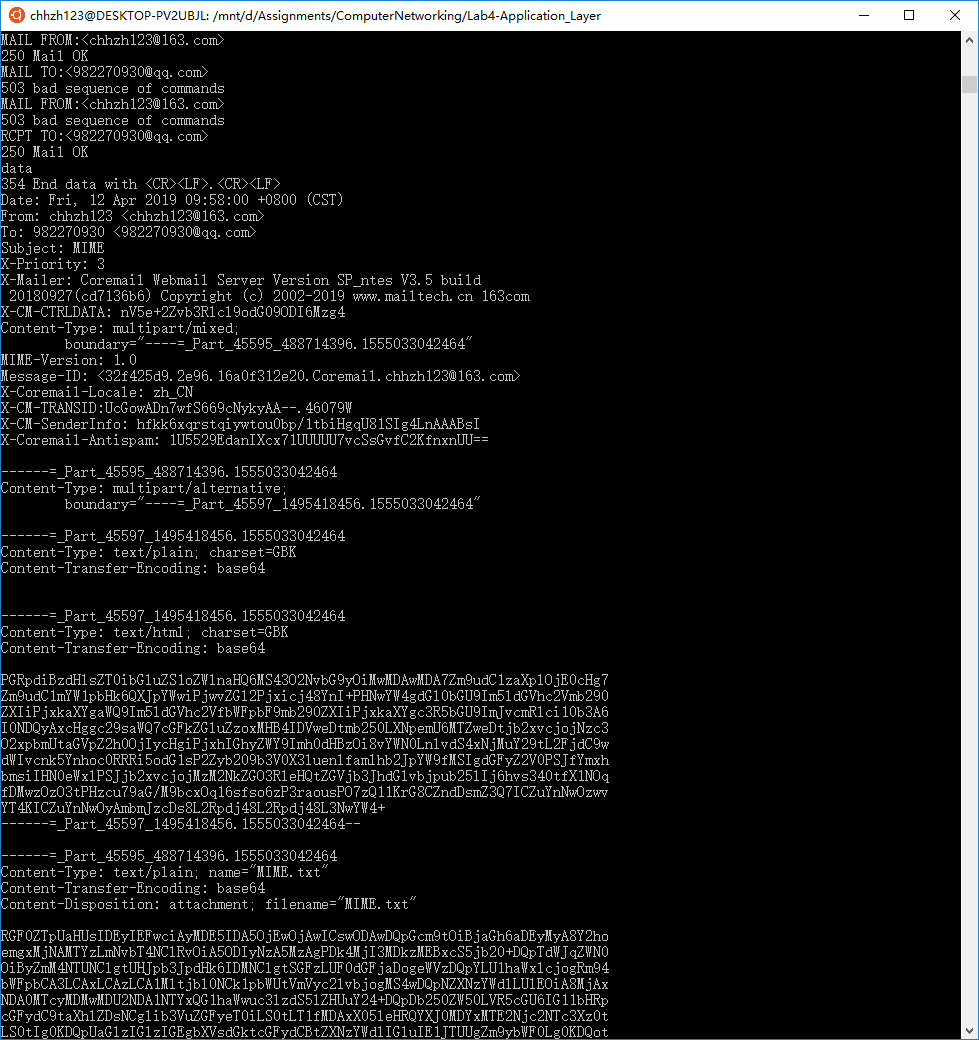
\includegraphics[width=0.8\linewidth]{fig/smtp-3.PNG}
\end{figure}
\begin{figure}[H]
\centering

\includegraphics[width=0.2\linewidth]{fig/smtp-31.PNG}
\end{figure}

\item (选做)从你的邮箱发一份邮件到同学的邮箱。QQ邮箱见【注意事项】。\\
请求和响应信息:
\begin{figure}[H]
\centering
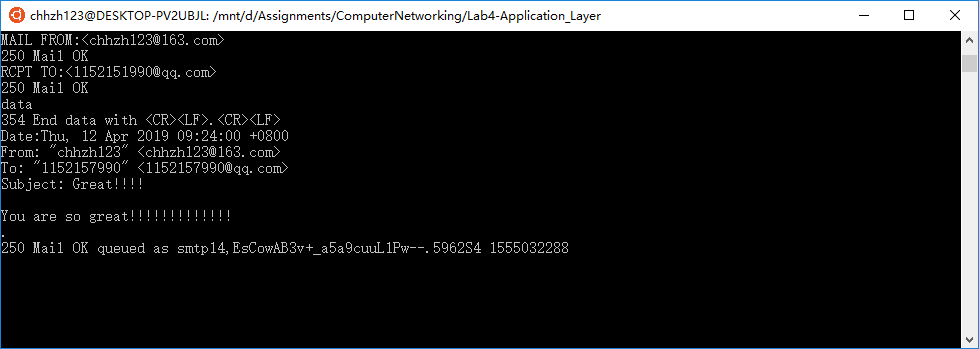
\includegraphics[width=0.8\linewidth]{fig/smtp-4.PNG}
\end{figure}
\begin{figure}[H]
\centering

\includegraphics[width=0.2\linewidth]{fig/smtp-41.PNG}
\end{figure}

\end{enumerate}

\subsection{POP3协议}
看完POP3协议的课件后做以下实验。
\par 邮箱\verb'zsureceiver3@sina.com'的用户名\verb'zsureceiver3',密码:\verb'123456Aa'。
\begin{enumerate}
\item 查看邮箱中每个邮件大小。\\
请求和响应信息:
\begin{figure}[H]
\centering
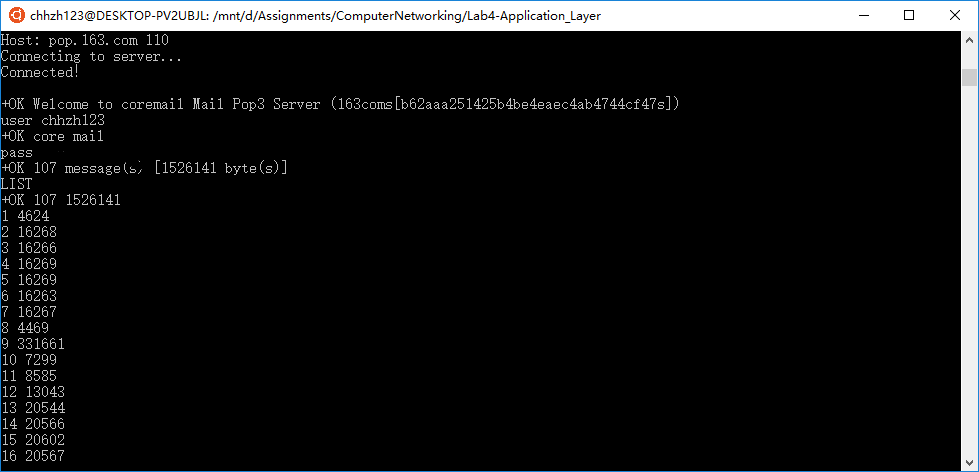
\includegraphics[width=0.8\linewidth]{fig/pop-1.PNG}
\end{figure}

\item 取回\verb'zsureceiver3@sina.com'最后一封邮件的邮件唯一标识符。\\
请求和响应信息:
\begin{figure}[H]
\centering
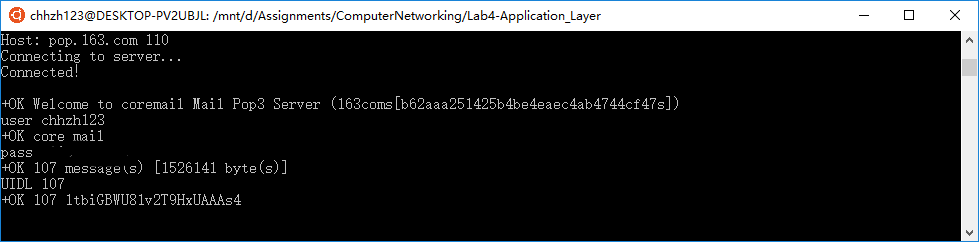
\includegraphics[width=0.8\linewidth]{fig/pop-2.PNG}
\end{figure}

\item 取回\verb'zsureceiver3@sina.com'最后一封邮件。\\
请求和响应信息:
\begin{figure}[H]
\centering
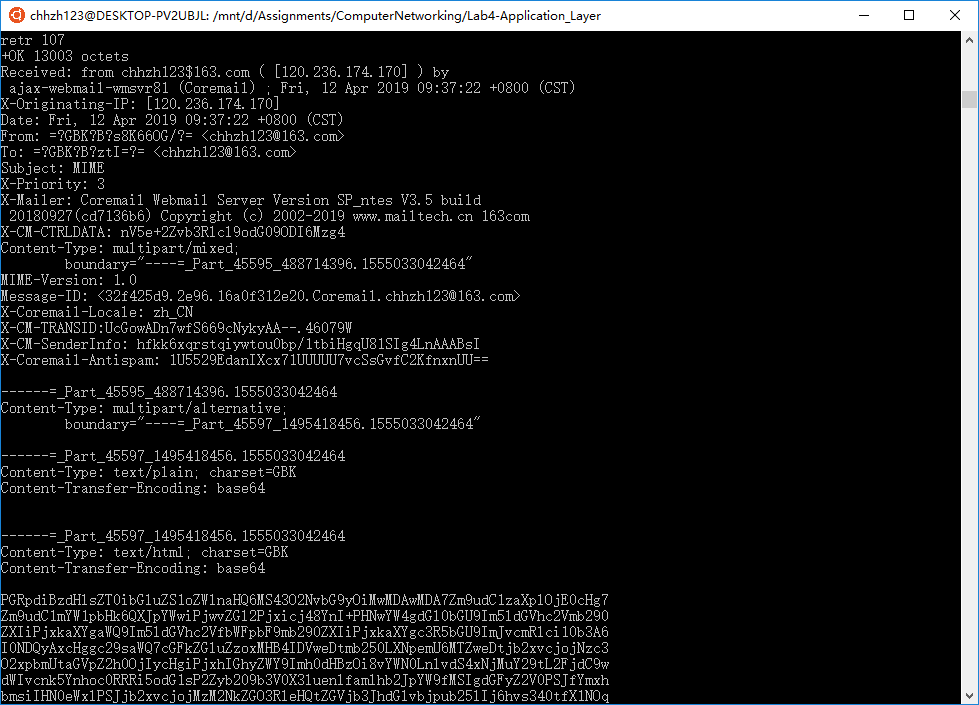
\includegraphics[width=0.8\linewidth]{fig/pop-3.PNG}
\end{figure}


\item 取回三(1)中发到你邮箱的邮件。QQ邮件见【注意事项】。\\
请求和响应信息:
\begin{figure}[H]
\centering
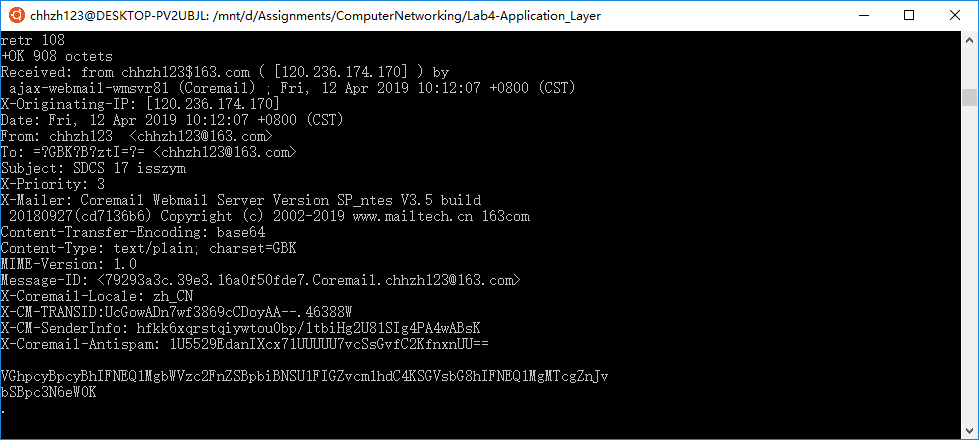
\includegraphics[width=0.8\linewidth]{fig/pop-4.PNG}
\end{figure}

\end{enumerate}

\subsection{FTP客户端}
编写一个程序(聊天程序的客户端),用FTP协议下载指定文件(选做)

源代码:
\begin{lstlisting}
#include <stdio.h>
#include <stdlib.h>
#include <sys/types.h>
#include <sys/socket.h>
#include <netinet/in.h>
#include <arpa/inet.h>
#include <netdb.h>
#include <unistd.h>
#include <string.h>
#include <error.h>
#include <pthread.h>

#define BUF_LEN 100000

void* receive(void* arg);

int main(int argc, char *argv[])
{
    /* check command line arguments */
    if (argc != 4) {
       fprintf(stderr,"usage: %s <hostname> <filename> <dstname>\n", argv[0]);
       exit(0);
    }
    struct hostent *server;
    char* hostname = argv[1];
    int port = 21; // ftp
    printf("Host: %s %d\n", hostname, port);
    char* filename = argv[2];
    char* dstname = argv[3];
    FILE *fp = fopen(dstname,"w");

    /* gethostbyname: get the server's DNS entry */
    server = gethostbyname(hostname);
    if (server == NULL) {
        fprintf(stderr,"Error: no such host as %s\n", hostname);
        exit(0);
    }

    struct  sockaddr_in sin;           /* an Internet endpoint address */
    char    buf[BUF_LEN+1];            /* buffer for one line of text  */
    char    res[BUF_LEN+1];
    int     sock;                      /* socket descriptor            */
    int     cc;                        /* recv character count         */

    // create socket
    sock = socket(PF_INET, SOCK_STREAM, IPPROTO_TCP);
    if (sock < 0) 
        perror("Error: opening socket\n");

    memset(&sin, 0, sizeof(sin));
    sin.sin_family = AF_INET;
    // sin.sin_addr.s_addr = inet_addr(host);
    bcopy((char *)server->h_addr,(char *)&sin.sin_addr.s_addr, server->h_length);
    sin.sin_port = htons((u_short)port);
    printf("Connecting to server...\n");
    int ret = connect(sock, (struct sockaddr *)&sin, sizeof(sin));
    if (ret == 0)
        printf("Connected!\n\n");
    else {
        perror("Error: Fail!\n");
        abort();
    }

    cc = recv(sock,buf,BUF_LEN, 0);
    buf[cc] = '\0';
    printf("%s", buf);

    memset(res, 0, sizeof(sin));
    strcpy(buf,"user abc\r\n");
    cc = send(sock,buf,strlen(buf),0);
    cc = recv(sock,buf,BUF_LEN, 0);
    buf[cc] = '\0';
    printf("user abc\r\n");
    printf("%s", buf);

    strcpy(buf,"pass 123666\r\n");
    cc = send(sock,buf,strlen(buf),0);
    cc = recv(sock,buf,BUF_LEN, 0);
    buf[cc] = '\0';
    printf("pass 123666\r\n");
    printf("%s", buf);

    strcpy(buf,"pasv\r\n");
    cc = send(sock,buf,strlen(buf),0);
    cc = recv(sock,buf,BUF_LEN, 0);
    buf[cc] = '\0';
    printf("pasv\r\n");
    printf("%s", buf);

    int addr_ftp[6];
    sscanf(buf, "%*[^(](%d,%d,%d,%d,%d,%d)",&addr_ftp[0],&addr_ftp[1],&addr_ftp[2],&addr_ftp[3],&addr_ftp[4],&addr_ftp[5]);

    struct  sockaddr_in r_sin;           /* an Internet endpoint address */
    int     r_sock;                      /* socket descriptor            */
    memset(&r_sin, 0, sizeof(r_sin));
    r_sock = socket(PF_INET, SOCK_STREAM, IPPROTO_TCP);
    r_sin.sin_family = AF_INET;
    // sin.sin_addr.s_addr = inet_addr(host);
    bcopy((char *)server->h_addr,(char *)&r_sin.sin_addr.s_addr, server->h_length);
    r_sin.sin_port = htons((u_short)(addr_ftp[4]*256 + addr_ftp[5]));
    printf("Connecting to data link %d.%d.%d.%d %d...\n",addr_ftp[0],addr_ftp[1],addr_ftp[2],addr_ftp[3],r_sin.sin_port);
    ret = connect(r_sock, (struct sockaddr *)&r_sin, sizeof(r_sin));
    if (ret == 0)
        printf("Connected!\n\n");
    else {
        perror("Error: Fail!\n");
        abort();
    }

    strcpy(buf,"retr ");
    strcat(buf,filename);
    strcat(buf,"\r\n");
    cc = send(sock,buf,strlen(buf),0);
    printf("%s",buf);
    cc = recv(sock,buf,BUF_LEN, 0);
    buf[cc] = '\0';
    printf("%s", buf);

    pthread_t pt;
    pthread_create(&pt,NULL,receive,&sock);

    printf("Begin downloading...\n");
    while (1){
        int cc = recv(r_sock, buf, BUF_LEN, 0);
        if (cc <= 0){
            // perror("Error: Server!\n");
            break;
        }
        buf[cc] = '\0';
        fprintf(fp, "%s", buf);
    }
    fclose(fp);
    printf("Finish downloading.\n");

    strcpy(buf,"quit\r\n");
    cc = send(sock,buf,strlen(buf),0);
    cc = recv(sock,buf,BUF_LEN, 0);
    buf[cc] = '\0';
    printf("quit\r\n");
    printf("%s", buf);

    close(sock);

    getchar();
    return 0;
}

void* receive(void* arg)
{
    char buf[BUF_LEN+1];
    int* sock = (int*) arg;
    while (1){
        int cc = recv(*sock, buf, BUF_LEN, 0);
        if (cc <= 0){
            // perror("Error: Server!\n");
            break;
        }
        buf[cc] = '\0';
        printf("%s", buf);
    }
    pthread_exit(0);
}
\end{lstlisting}

运行截屏:
\begin{figure}[H]
\centering
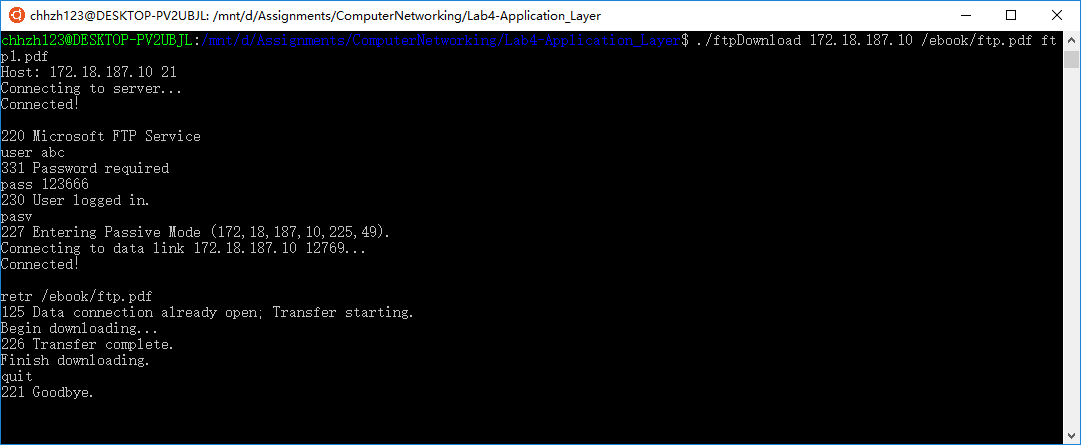
\includegraphics[width=0.8\linewidth]{fig/ftp-download.PNG}
\end{figure}

\subsection{多线程TCP客户端}
采用聊天程序的客户端。该客户端采用两个进程实现:一个输入和发送线程,一个接收线程。(选做)

源代码:
\begin{lstlisting}
#include <stdio.h>
#include <stdlib.h>
#include <sys/types.h>
#include <sys/socket.h>
#include <netinet/in.h>
#include <arpa/inet.h>
#include <netdb.h>
#include <unistd.h>
#include <string.h>
#include <error.h>
#include <pthread.h>

#define BUF_LEN 100000

void* receive(void* arg);

int main(int argc, char *argv[])
{
    /* check command line arguments */
    if (argc != 3) {
       fprintf(stderr,"usage: %s <hostname> <port>\n", argv[0]);
       exit(0);
    }
    struct hostent *server;
    char* hostname = argv[1];
    int port = atoi(argv[2]);
    printf("Host: %s %d\n", hostname, port);

    /* gethostbyname: get the server's DNS entry */
    server = gethostbyname(hostname);
    if (server == NULL) {
        fprintf(stderr,"Error: no such host as %s\n", hostname);
        exit(0);
    }

    struct  sockaddr_in sin;           /* an Internet endpoint address */
    char    buf[BUF_LEN+1];            /* buffer for one line of text  */
    char    res[BUF_LEN+1];
    int     sock;                      /* socket descriptor            */
    int     cc;                        /* recv character count         */

    // create socket
    sock = socket(PF_INET, SOCK_STREAM, IPPROTO_TCP);
    if (sock < 0) 
        perror("Error: opening socket\n");

    memset(&sin, 0, sizeof(sin));
    sin.sin_family = AF_INET;
    // sin.sin_addr.s_addr = inet_addr(host);
    bcopy((char *)server->h_addr,(char *)&sin.sin_addr.s_addr, server->h_length);
    sin.sin_port = htons((u_short)port);
    printf("Connecting to server...\n");
    int ret = connect(sock, (struct sockaddr *)&sin, sizeof(sin));
    if (ret == 0)
        printf("Connected!\n\n");
    else {
        perror("Error: Fail!\n");
        abort();
    }

    pthread_t pt;
    pthread_create(&pt,NULL,receive,&sock);

    memset(res, 0, sizeof(sin));
    while (1){
        gets(buf);
        strcat(buf,"\r\n");
        cc = send(sock,buf,strlen(buf),0);
    }

    close(sock);

    getchar();
    return 0;
}

void* receive(void* arg)
{
    char buf[BUF_LEN+1];
    int* sock = (int*) arg;
    while (1){
        int cc = recv(*sock, buf, BUF_LEN, 0);
        if (cc <= 0){
            perror("Error: Server!\n");
            abort();
            break;
        }
        buf[cc] = '\0';
        printf("%s\n", buf);
    }
    pthread_exit(0);
    abort();
}
\end{lstlisting}


\section{完成情况}
是否采用了老师的\verb'TcpClient.exe'执行命令:[\xmark]

是否完成以下步骤?(\cmark 完成\quad\xmark 未做)
\par 1. [\cmark]\qquad 2. [\cmark]\qquad 3.[\cmark]
\par 4. [\cmark]\qquad 5. [\cmark]\qquad 6.[\cmark]

\section{实验体会}
% 写出实验过程中遇到的问题,解决方法和自己的思考;并简述实验体会(如果有的话)。

本次实验由于有之前实验编写的TCP客户端,所以在其基础上进行一定修改即可完成HTTP、FTP、SMTP、POP等功能。
但最麻烦的是各种各种协议的编写规则,一开始就被HTTP协议卡了很久,因为发送的信息最后没有添加两个\verb'\r\n',导致服务器端以为还有消息要接收进而没有进行处理,客户端就没有收到消息。
同时还有Linux环境下的编码问题,收到的信息经常无法正常显示,但后来通过不断尝试终于得到部分解决。

\end{document}
% 【交实验报告】
% (1) 每位同学单独完成本实验内容并填写实验报告。
% (2) 上交网址:http://172.18.187.9/netdisk/default.aspx?vm=17net  实验上交/编程实验
% (3) 截止日期(不迟于):2019年4月14日 23:00 (周日)。
% 上传文件:学号_姓名_应用层实验报告.doc   (不要用PDF文件)
%           学号_姓名_应用层实验报告.rar  (如果采用自己编写的TCPClient完成实验,打包源代码和可执行文件,选做的源代码也打包进去)